\subsection{ASIC}

\subsubsection{Netlist} Une fois la conception réalisée à l'aide de langages de
description matérielle, on peut obtenir une netlist du circuit intégré. Cette
netlist contient dans un premier temps une liste qui définit les composants utilisés
dans ce circuit intégré. Chaque composant est défini par les différents points de
connexion (appelé \textit{ports}) qu'il possède et par ses propriétés élémentaires. Un
composant peut être quelque chose d'élémentaire comme un transistor ou une résistance
tout comme un circuit intégré complexe. Ensuite la netlist va alors décrire des
connexions entre des composants. Chaque composant décrit dans le réseau est forcément
un des composants de la liste précédemment décrite, on dit alors que ce composant est
une instance de la définition donnée dans la liste de composants. Les connexions sont
décrites par une liste de fils. Un fil connecte un port donné d'une instance avec un
autre port donné d'une autre instance. Pour limiter la redondance, on peut
hiérarchiser les netlists, c'est à dire que l'on peut ranger une partie d'un réseau
dans une définition d'un composant. De cette manière, si cette partie est répétée
plusieurs fois dans le réseau, on peut l'insérer comme on insérerait un composant
élémentaire, et la description de cette partie n'est alors donnée qu'une seule fois.

\subsubsection{Fabrication d'ASIC}

\begin{figure}[hb]
\begin{center}
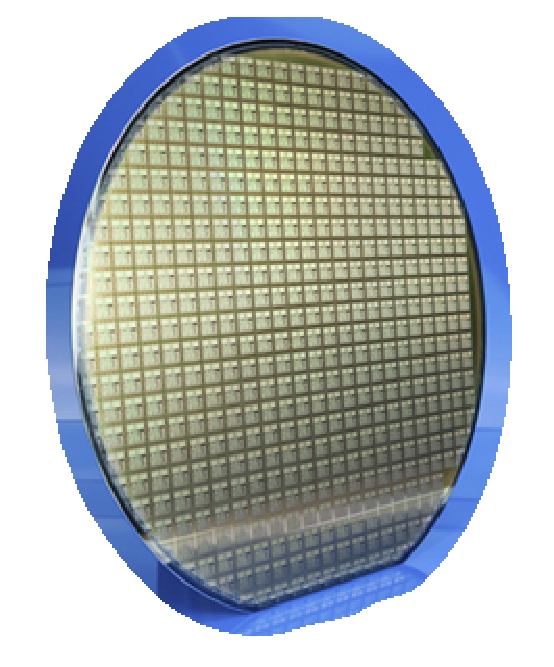
\includegraphics[scale=0.4]{asic.eps}
\end{center}
\caption{Waffer comportant plusieurs ASIC (image récupérée sur \url{http://tes-dst.com/tes-dst/services/asic-design-service/asic-design-library-a-ip.html})}
\end{figure}

À partir de la description en netlist, il est possible d'obtenir un fichier
(généralement au format GDSII) qui représente le dessin physique du circuit intégré.
C'est-à-dire qu'il représente entre autre les formes géométriques à graver sur le
silicium. C'est ce fichier qui est envoyé aux fondeurs pour obtenir les masques nécessaires à la gravure du système. Ce procédé utilisant le
plus souvent la lithographie est très complexe et ne sera pas détaillé dans ce
rapport. La fabrication d'ASIC demande un fort investissement en matériel, c'est
pour cela qu'on observe une séparation entre les entreprises qui conçoivent les
circuits intégrés et les fonderies car il faut une très grande production pour
amortir les investissements. Seules quelques entreprises telles qu'Intel,
STMicroelectronics, Texas Instruments qui produisent de très grands volumes peuvent
se permettre de faire en même temps la conception et la réalisation de leurs
circuits. Les ASIC ne peuvent alors être réalisés pour un prix raisonnable en petit
volume.


\subsection{FPGA}

\begin{figure}[h!]
\begin{center}
\includegraphics[scale=0.1]{fpga.eps}
\end{center}
\caption{Une carte de developpement équipé d'un FPGA (image récupérée sur \url{http://www.dlpdesign.com/fpga/fpga.shtml})}
\end{figure}

Les FPGA (\textit{Field Programmable Gate Array}) sont des circuits logiques
programmables. En effet, \textit{Field Programmage} signifie programmable sur le champ,
le circuit peut être programmé après sa fabrication pour réaliser n'importe quelle
fonction logique. La configuration d'un FPGA est obtenue à l'aide de langages HDL
qui permettent aussi de concevoir les ASIC, c'est pour cela que les FPGA peuvent être
utilisés pour faire des prototypes d'ASIC.

Les FPGA sont constitués d'un nombre très importants de blocs logiques rangés en
matrice (d'où le terme \textit{Gate Array} de FPGA). Ces blocs logiques peuvent être
configurés pour effectuer des fonctions logiques élémentaires (et, ou, ou exclusif,
non) ou quelques fonctions logiques plus complexes. Ils peuvent aussi être configurés
en bascules ou en d'autres éléments permettant de mémoriser de l'information. Ces
bloques logiques peuvent également être connectés de manière arbitraire entre eux.
C'est en définissant les fonctions réalisées par ces blocs logiques et des
connexions entre eux que l'on peut configurer un FPGA pour obtenir le fonctionnement
attendu. Cette configuration est générée de manière automatique à partir de
description en HDL. De nos jours, le nombre de blocs logiques sur les FPGA se compte
en millions. 

Les cartes FPGA contiennent en plus du réseau de blocs logiques programmables des
périphériques. Cela permet d'économiser des portes. De plus certains périphériques
tels que les GPIO ne peuvent pas être programmés à l'aide de blocs logiques. Il
n'est donc pas rare de voir des cartes FPGA embarquer des GPIO, de la RAM, des
cartes réseaux. Dans notre projet tutoré, la différence des
périphériques de la Nexys3 utilisée à l'INSA et ceux de \textit{Milkymist} entrainent des problèmes de portabilité.

\begin{figure}
\begin{center}
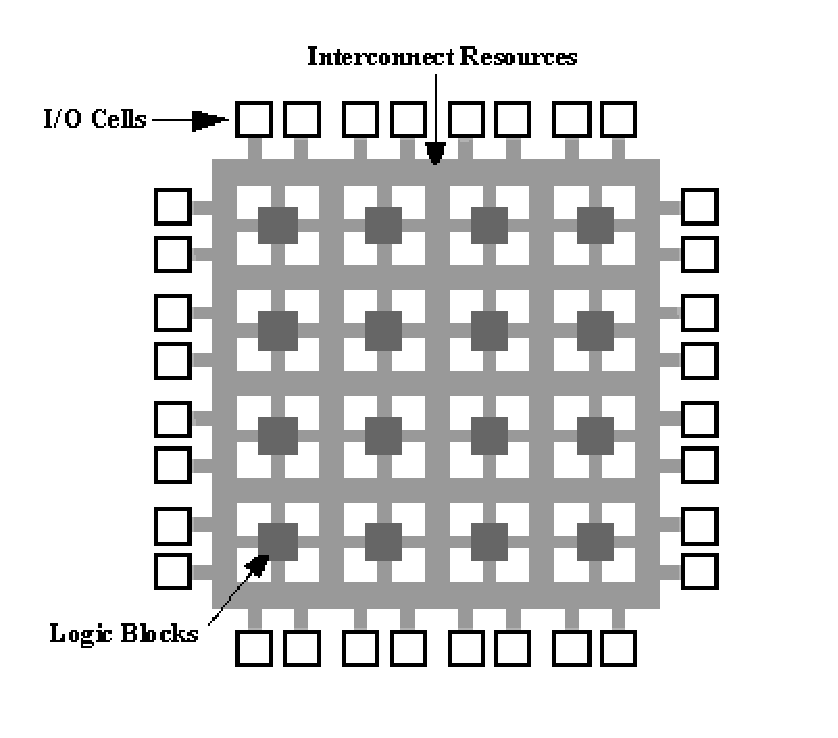
\includegraphics[scale=0.5]{porte.eps}
\end{center}
\caption{Schéma représentant la structure en matrice des portes d'un FPGA (image récupérée sur \url{http://proxacutor.free.fr/})}
\end{figure}
